\newprob{1719147035}
{
    % act physcs p253 q1
    關於電場和磁場的敍述,哪一個是正確的?
    \begin{tasks}
        \task 兩者能吸引和排斥靜止的電荷。
        \task 兩者能偏轉運動中的電荷。
        \task 兩者的場力線能以閉合的環表示。
        \task 兩者能沿着場力線的切線方向施力。
    \end{tasks}
}{B}

\newprob{1719147391}
{
    % act physcs p253 q2
    圖示為兩根磁棒之間的磁場。下列哪些敘述是正 確的?
    \par{\par\centering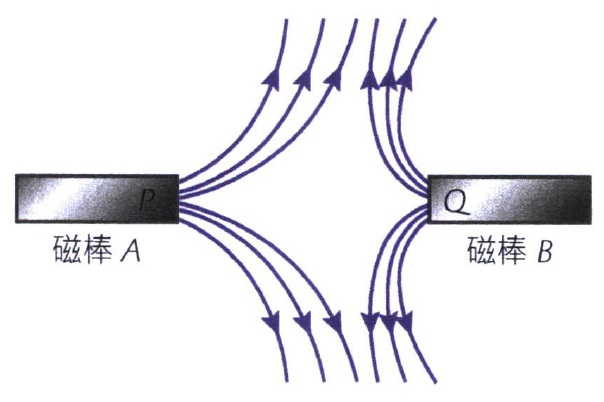
\includegraphics[width=.35\textwidth]{./img/ch4_magnetostatics_mc_2024-06-23-20-56-53.png}\par}
    \begin{statements}
        \task 在兩極P和Q之間有一個中和點。
        \task 磁棒 A 比磁棒B 強。
        \task 兩極P和Q皆為磁南極。
    \end{statements}
    \begin{tasks}
        \task 只有(1)和(2)
        \task 只有(1)和(3)
        \task 只有(2)和(3)
        \task (1), (2) 和 (3)
    \end{tasks}
}{A}

\newprob{1719147544}
{
    % act physcs p253 q3
    一條銅導線繞在一個軟鐵心上,成為一個電磁 鐵,用來提起一些鐵製物件。以下哪些方法能增 加電磁鐵的強度?
    \par{\par\centering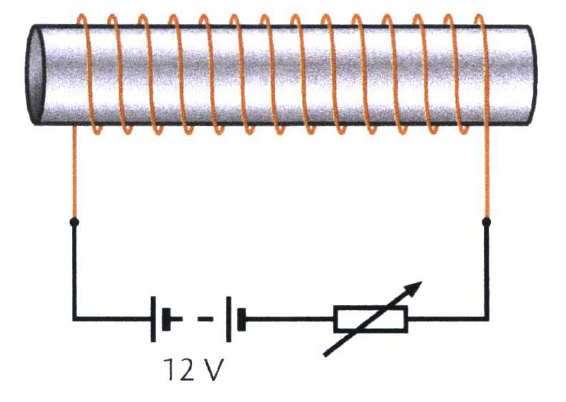
\includegraphics[width=.35\textwidth]{./img/ch4_magnetostatics_mc_2024-06-23-20-59-43.png}\par}

    \begin{statements}
        \task 把線圈繞在另一個較大的軟鐵心上,但保持 螺線管長度和線圈匝數不變。
        \task 增加線圈數目,但保持螺線管長度不變。
        \task 把12V 電池組換成24V 電池組。
    \end{statements}
    \begin{tasks}
        \task 只有(1)
        \task 只有(2)
        \task 只有(1)和(3)
        \task 只有(2)和(3)
    \end{tasks}
}{D}

\newprob{1719147629}
{
    % act physcs p253 q4
    兩個完全相同的長螺線管載有相同的電流。當兩 者相距較遠時,每個螺線管一端的磁場為B。
    \par{\par\centering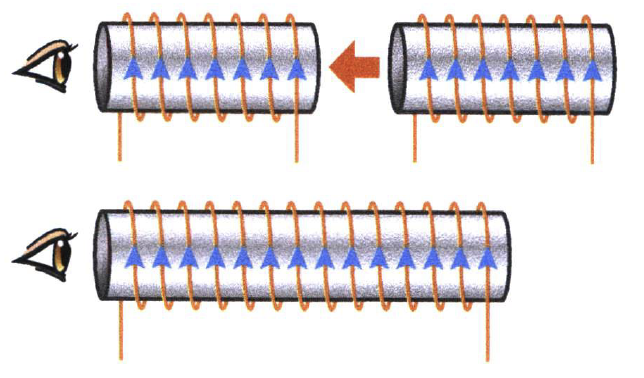
\includegraphics[width=.35\textwidth]{./img/ch4_magnetostatics_mc_2024-06-23-21-00-53.png}\par}
    現在,兩個螺線管靠近並合二為一,如圖。對這 新的螺線管,接近觀察者的一端為磁北極(N)還 是磁南極(S)?這端的磁場量值又為多少?
    \begin{tasks}
        \task \textbf{磁極}\tab \tab \textbf{量值}
        \task N \tab \tab B
        \task N \tab \tab 2B
        \task S \tab \tab B
        \task S \tab \tab 2B
    \end{tasks}

}{A}

\newprob{1719147749}
{
    % act physcs p253 q5
    一個載電流的長方形線圈 PQRS 如下圖般放在一 個匀強磁場中。在圖示的一刻,磁場與線圈的平 面互相垂直。下列哪些敍述是正確的?
    \par{\par\centering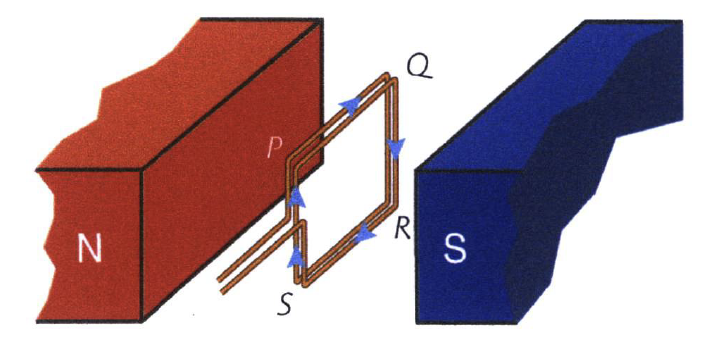
\includegraphics[width=.35\textwidth]{./img/ch4_magnetostatics_mc_2024-06-23-21-02-39.png}\par}
    \begin{statements}
        \task 一道磁力作用在線圈QR一側。
        \task 磁力傾向縮小線圈的面積。
        \task 若線圈稍受干擾,仍會返回原來位置。
    \end{statements}
    \begin{tasks}
        \task 只有(1)和(2)
        \task 只有(1)和(3)
        \task 只有(2)和(3)
        \task (1), (2) 和 (3)
    \end{tasks}
}{A}

\newprob{1719147805}
{
    % act physcs p253 q6
    一顆帶電粒子沿一個螺線管的中軸投進管內。若 螺線管通以交流電,
    \begin{tasks}
        \task 粒子進行圓周運動。
        \task 粒子在螺線管中軸上前後振盪。
        \task 粒子進行匀加速運動。
        \task 粒子進行匀速運動。
    \end{tasks}
}{D}

\newprob{1719147843}
{
    % act physcs p253 q7
    一顆電荷以直角進入一個匀強磁場,並在垂直於 磁場的平面上進行圓周運動。以下哪一幅線圈最 能表示運動的週期T與圓形路徑半徑$r$之間的關 係?
    \begin{tasks}(2)
        \task \topalign{\par\centering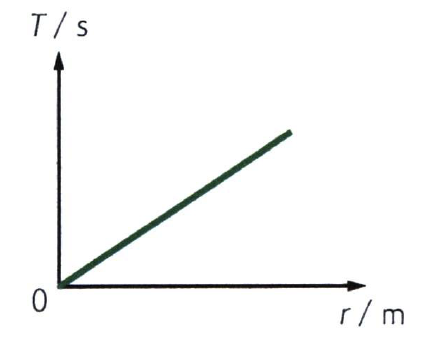
\includegraphics[width=.25\textwidth]{./img/ch4_magnetostatics_mc_2024-06-23-21-04-37.png}\par}
        \task \topalign{\par\centering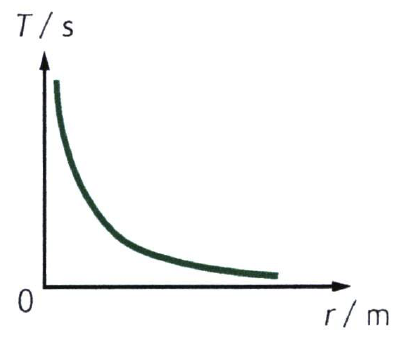
\includegraphics[width=.25\textwidth]{./img/ch4_magnetostatics_mc_2024-06-23-21-04-43.png}\par}
        \task \topalign{\par\centering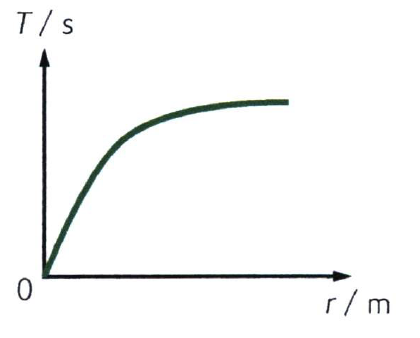
\includegraphics[width=.25\textwidth]{./img/ch4_magnetostatics_mc_2024-06-23-21-04-49.png}\par}
        \task \topalign{\par\centering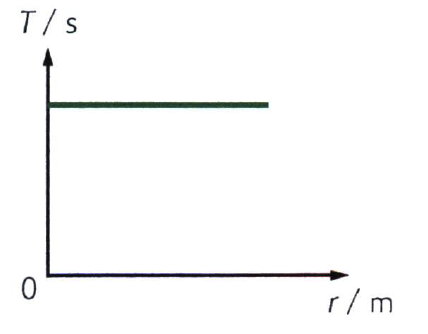
\includegraphics[width=.25\textwidth]{./img/ch4_magnetostatics_mc_2024-06-23-21-04-55.png}\par}
    \end{tasks}
}{D}

